\documentclass[11pt,a4paper]{article}
\usepackage[utf8]{inputenc}
\usepackage[T1]{fontenc}
\usepackage{graphicx}
\usepackage{booktabs}
\usepackage{hyperref}
\usepackage{amsmath}
\usepackage{siunitx}
\usepackage{geometry}
\usepackage{caption}
\usepackage{subcaption}
\usepackage{float}
\geometry{margin=2.5cm}

\title{Preliminary Protocol Choices for CAMPUS 5G Device--Edge Communication\\[0.3em]
\large Benchmarking gRPC, Zenoh, and MQTT under Emulated 5G Conditions}
\author{Samiullah Khairy}
\date{May 26, 2026}

\begin{document}
\maketitle

\section{What this is about}

For the CAMPUS project, I needed to evaluate which protocol to use for the bidirectional device--edge communication layer (covering both the downlink from the edge server and the uplink/acknowledgements from the devices). The three candidates are:

\begin{itemize}
    \item \textbf{gRPC} (over HTTP/2) --- the edge server opens a direct bidirectional stream to each OBU. No broker in the middle. Uses Protocol Buffers for serialization.
    \item \textbf{Zenoh} --- a pub/sub protocol designed for IoT and robotics. Traffic goes through a lightweight Zenoh router, but the routing layer is thin compared to a traditional message broker.
    \item \textbf{MQTT} (Mosquitto broker, QoS~1) --- the standard IoT pub/sub protocol. All traffic passes through a central Mosquitto broker. I used QoS~1 (at-least-once delivery with PUBACK acknowledgement).
\end{itemize}

The goal was to measure round-trip latency (RTT) as I scale the number of devices and degrade the network link, to see which protocol holds up for real-time safety applications.

\section{How the experiments were set up}

\subsection{Containerized testbed}

Each experiment runs entirely in Docker. The edge server, the broker/router (if applicable), and each simulated OBU are separate containers connected on a shared bridge network (\texttt{campus-net}). So when I say ``$N=10$ devices'', that means 10 separate device containers plus the server-side containers, all running simultaneously on the same host.

The communication pattern is the same across all three protocols:
\begin{enumerate}
    \item The edge server publishes a command message to each device (containing a timestamp and a payload).
    \item The device receives the command, echoes back an acknowledgement containing the original timestamp.
    \item The edge server receives the ack and computes the round-trip time from its original send timestamp.
\end{enumerate}

All timestamps use \texttt{time.monotonic\_ns()} (monotonic clock) to avoid issues with NTP clock adjustments during a run. The edge server waits 5 seconds before starting to send data, which gives the matrix runner time to inject the network impairment rules before any packets flow.

\subsection{Network impairment}

I used the Linux kernel's Traffic Control (\texttt{tc netem}) to inject delay, jitter, and packet loss directly on each container's \texttt{eth0} interface. This requires \texttt{iproute2} installed in the container and \texttt{cap\_add: [NET\_ADMIN]} in the compose file.

Three profiles were tested:

\begin{table}[H]
\centering
\caption{Network impairment profiles}
\label{tab:profiles}
\begin{tabular}{llll}
\toprule
Profile & One-way delay & Jitter (normal dist.) & Packet loss \\
\midrule
\texttt{clean} & 0 ms & 0 ms & 0\% \\
\texttt{good\_5g} & 20 ms & 1 ms & 0.1\% \\
\texttt{degraded\_5g} & 80 ms & 10 ms & 1.0\% \\
\bottomrule
\end{tabular}
\end{table}

Since the delay is applied on both the edge and device containers, the theoretical minimum RTT for \texttt{good\_5g} is $2 \times 20 = 40$~ms, and for \texttt{degraded\_5g} it is $2 \times 80 = 160$~ms.

\textbf{Note:} These are synthetic impairments on a Docker bridge network. They don't capture real gNodeB scheduling, HARQ retransmissions, or RLC layer behavior. The numbers here tell us about protocol-level overhead and queuing behavior, not about actual 5G radio performance. The plan is to validate these findings on the live 5G testbed in the next phase.

\subsection{Sweep matrix}

Each configuration was run for 30 seconds. The full matrix sweeps:

\begin{itemize}
    \item 3 protocols $\times$ 3 network profiles $\times$ 4 device counts ($N = 1, 2, 5, 10$) $\times$ 2 payload sizes (100~B, 2000~B) $\times$ 2 message rates (5~Hz, 10~Hz) = \textbf{144 runs total}.
\end{itemize}

At 10~Hz with $N=10$ devices over 30 seconds, this gives around 3000 RTT samples per run, which is enough for stable percentile estimates. Note that the reported loss percentage in the results is calculated as the ratio of expected ACKs that were not received within the 30-second experiment window. This metric includes both actual packet drops at the network level and messages that were still in flight or queued in the protocol layers when the experiment terminated.

\section{Results}

\subsection{Baseline: clean network}

On the local bridge network with no artificial delay, this measures pure protocol overhead --- serialization, socket processing, broker routing.

\begin{table}[H]
\centering
\caption{Baseline latency on clean network ($N=1$, 100~B, 10~Hz)}
\label{tab:baseline}
\begin{tabular}{lrrrr}
\toprule
Protocol & p50 (ms) & p95 (ms) & p99 (ms) & Mean (ms) \\
\midrule
Zenoh & 0.99 & 2.56 & 3.32 & 1.22 \\
gRPC  & 2.26 & 4.37 & 4.66 & 2.52 \\
MQTT  & 46.23 & 48.78 & 49.51 & 46.00 \\
\bottomrule
\end{tabular}
\end{table}

Zenoh and gRPC are both sub-5~ms. The interesting thing is MQTT: even with zero network delay, it shows a consistent $\sim$46~ms latency. This appears to be related to the \texttt{paho-mqtt} client's internal event loop scheduling combined with QoS~1 PUBACK roundtrip overhead; I did not isolate the individual contribution of each component. This is a client library implementation detail, not a protocol limitation --- but it's what you get out of the box with the standard Python client.

As I scale to $N=10$ on the clean network, gRPC's p95 rises to about 6--9~ms (expected, since 10 concurrent streams share CPU time), while Zenoh stays under 4~ms. MQTT generally stays flat at $\sim$47--50~ms regardless of $N$, dominated by the polling timeout. However, in the $N=10$, 100~B configuration, MQTT shows a bimodal latency distribution with the median (p50) dropping to $\sim$6--8~ms while the p95 remains at $\sim$49~ms. This appears to be a \texttt{paho-mqtt} scheduling artifact under high broker activity where the client loop thread processes queued messages more aggressively, bypassing the usual event loop sleep timeout, and warrants further investigation.

\subsection{Good 5G conditions}

Under the \texttt{good\_5g} profile (40~ms theoretical RTT floor, 0.1\% loss), I'm checking whether the protocols can track the network delay without adding significant overhead on top.

\begin{table}[H]
\centering
\caption{Latency under good 5G conditions (2000~B payload, 10~Hz)}
\label{tab:good5g}
\begin{tabular}{lcrrrrr}
\toprule
Protocol & $N$ & Loss (\%) & p50 (ms) & p95 (ms) & p99 (ms) \\
\midrule
Zenoh & 5  & 4.3 & 43.45 & 45.97 & 47.11 \\
gRPC  & 5  & 4.7 & 43.13 & 46.58 & 48.93 \\
MQTT  & 5  & 3.4 & 87.07 & 94.13 & 128.81 \\
\midrule
Zenoh & 10 & 4.4 & 43.05 & 45.74 & 46.88 \\
gRPC  & 10 & 6.2 & 42.19 & 45.21 & 47.75 \\
MQTT  & 10 & 2.9 & 84.43 & 115.35 & 128.64 \\
\bottomrule
\end{tabular}
\end{table}

Zenoh and gRPC both sit right on the 40~ms floor. Even going from $N=5$ to $N=10$, their latencies barely move. MQTT is at about 84--87~ms (the 40~ms network RTT + the $\sim$45~ms client polling overhead), with tail latencies starting to creep up to 128~ms at $N=10$.

Figure~\ref{fig:latency_vs_n} shows how the p95 latency evolves as $N$ scales under these conditions.

\begin{figure}[H]
\centering
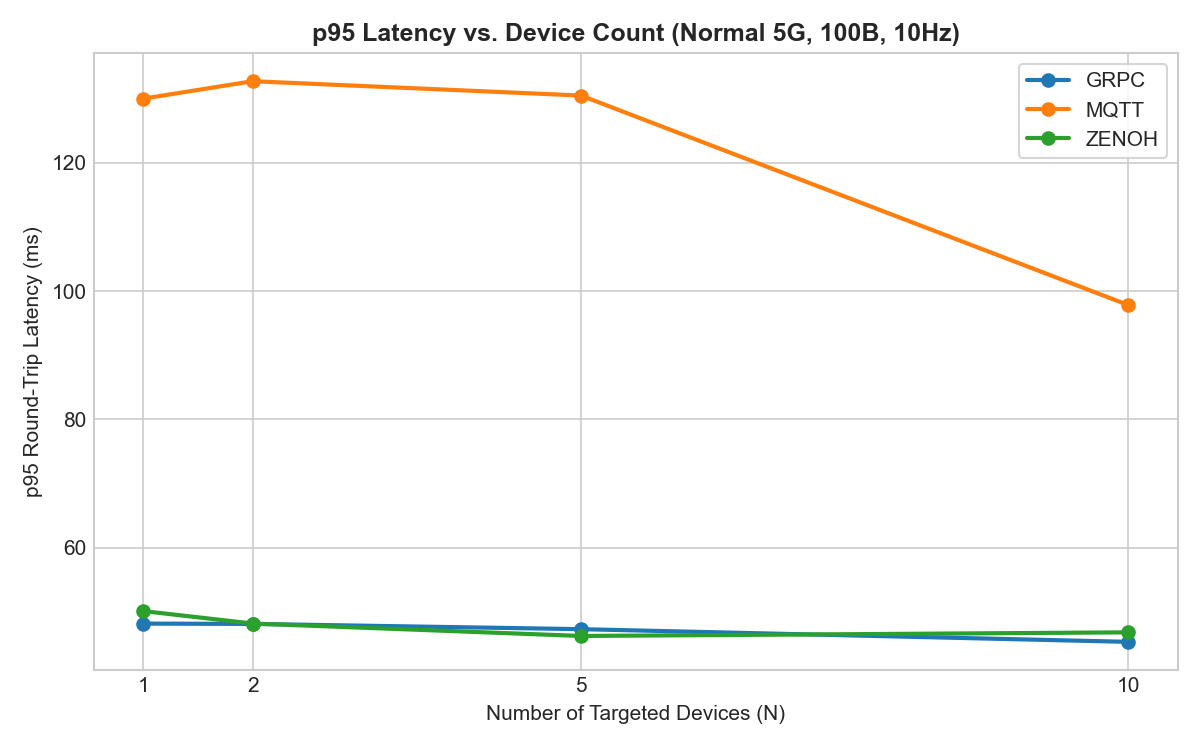
\includegraphics[width=0.75\textwidth]{results/matrix/latency_vs_N.png}
\caption{p95 latency vs.\ number of devices under good 5G (100~B, 10~Hz). Zenoh and gRPC stay flat; MQTT carries a constant offset from the polling delay.}
\label{fig:latency_vs_n}
\end{figure}

\subsection{Degraded 5G conditions --- where MQTT breaks}

This is where things get interesting. The \texttt{degraded\_5g} profile adds 160~ms RTT and 1\% packet loss. At 10~Hz with 10 devices, the edge server is pushing 100 messages per second through the network.

\begin{table}[H]
\centering
\caption{Latency under degraded 5G conditions (2000~B payload, 10~Hz)}
\label{tab:degraded5g}
\begin{tabular}{lcrrrrr}
\toprule
Protocol & $N$ & Loss (\%) & p50 (ms) & p95 (ms) & p99 (ms) \\
\midrule
Zenoh & 5  & 1.8 & 164.00 & 217.06 & 411.67 \\
gRPC  & 5  & 4.1 & 164.85 & 267.43 & 429.83 \\
MQTT  & 5  & 2.9 & 11{,}740 & 22{,}015 & 23{,}061 \\
\midrule
Zenoh & 10 & 1.8 & 164.28 & 282.93 & 440.10 \\
gRPC  & 10 & 5.7 & 164.01 & 305.37 & 444.23 \\
MQTT  & 10 & 4.0 & 31{,}957 & 58{,}370 & 61{,}375 \\
\bottomrule
\end{tabular}
\end{table}

Zenoh and gRPC handle it fine. Their median latency sits right at the 160~ms floor, and the p99 spikes to about 440~ms, which is just TCP doing its normal retransmission recovery when a packet gets lost. That's expected and acceptable.

MQTT is a different story. At $N=10$, the \textbf{median} latency is 32 seconds and the p95 is 58 seconds. The protocol is unusable.

At $N=5$ with the same payload at \textit{5~Hz} (half the message rate), MQTT's p50 is already 576~ms. At 10~Hz it jumps to 11.7 seconds. This highlights the nonlinear nature of the queue collapse under packet loss: doubling the message rate causes the median latency to jump by more than 20$\times$ as TCP retransmissions cascade and the broker queue fails to drain.

Figure~\ref{fig:cdf} shows the latency CDF, and Figure~\ref{fig:profile} compares the p95 across network profiles.

\begin{figure}[H]
\centering
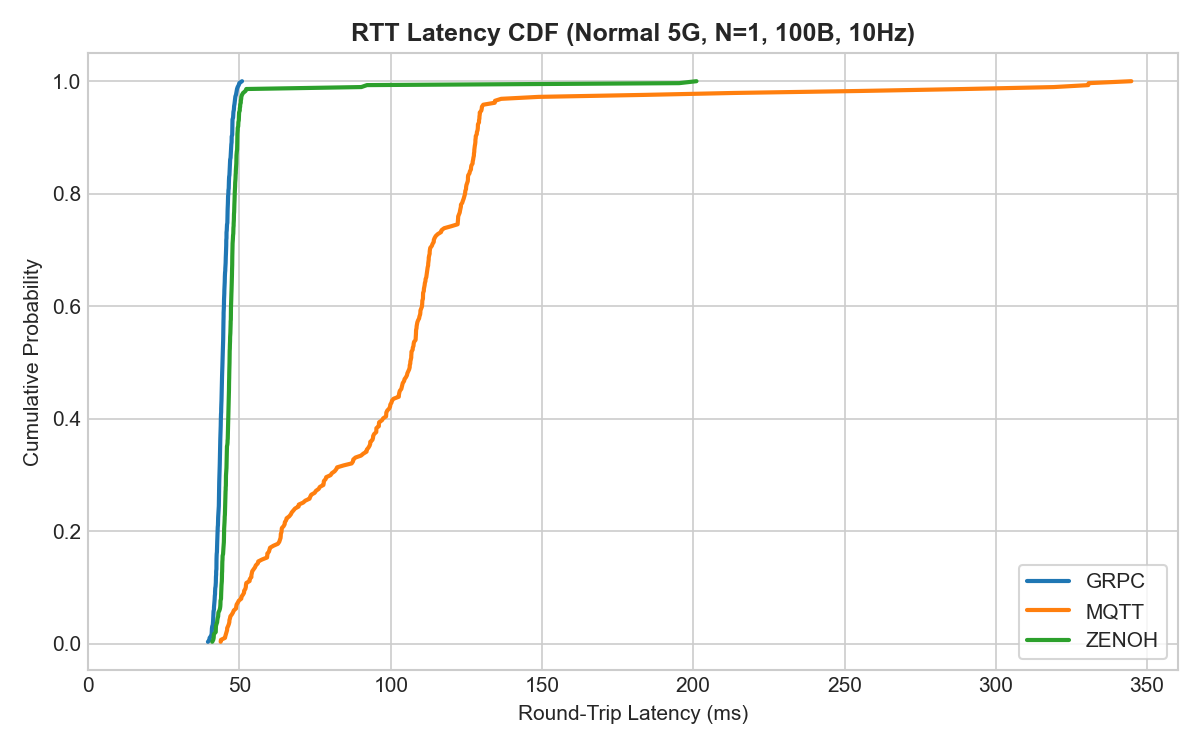
\includegraphics[width=0.75\textwidth]{results/matrix/latency_cdf.png}
\caption{RTT latency CDF under good 5G conditions. The MQTT curve is shifted right by $\sim$45~ms relative to gRPC and Zenoh.}
\label{fig:cdf}
\end{figure}

\begin{figure}[H]
\centering
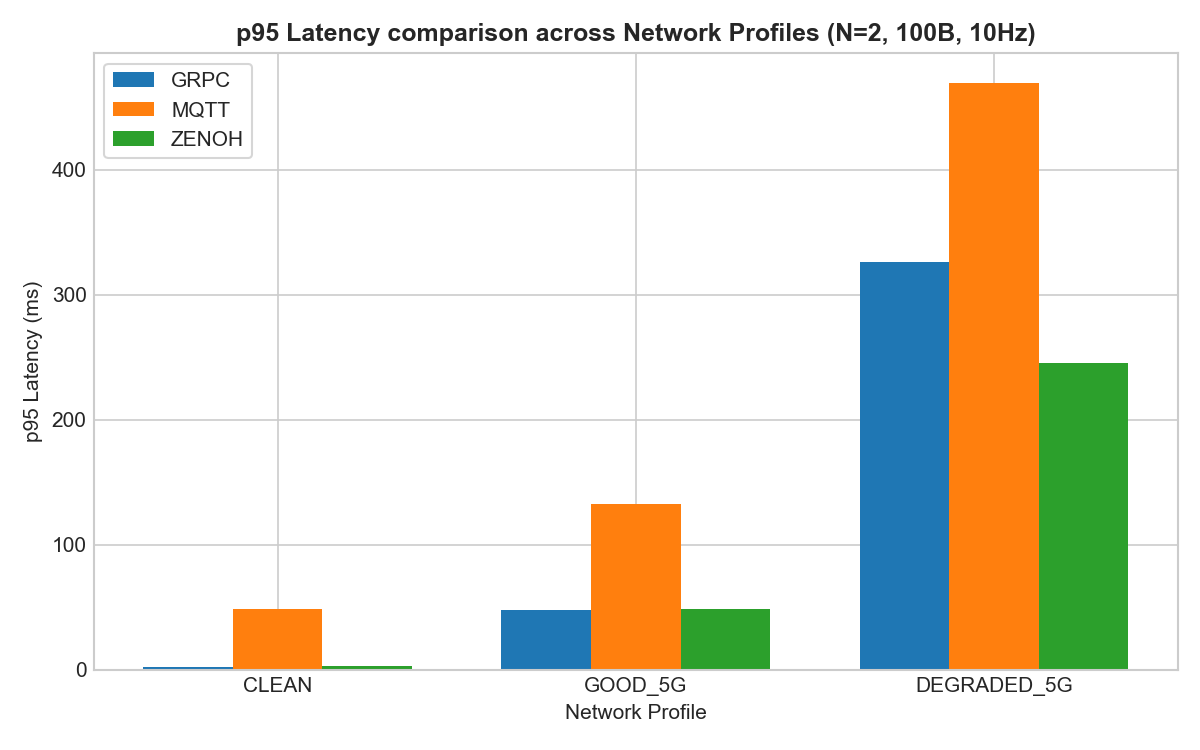
\includegraphics[width=0.75\textwidth]{results/matrix/profile_comparison.png}
\caption{p95 latency across network profiles ($N=2$, 100~B, 10~Hz).}
\label{fig:profile}
\end{figure}

\section{Why MQTT collapses under loss}

The root cause is straightforward: MQTT uses a central broker (Mosquitto). All messages from the edge server pass through the broker before being forwarded to the devices. Under QoS~1, the broker needs a \texttt{PUBACK} from the device before marking the message as delivered.

When 1\% of packets are lost on the link:
\begin{enumerate}
    \item TCP detects the loss and retransmits. During this time, the TCP send window shrinks and the socket blocks.
    \item The QoS~1 handshake stalls --- the broker is waiting for an ack that's stuck behind a TCP retransmission.
    \item Meanwhile, the edge server keeps publishing at 10~Hz. Those messages accumulate in the broker's internal queue.
    \item Once the broker queue starts to grow, the system enters a regime where new messages cannot drain faster than they arrive, and latency grows superlinearly until the run ends.
\end{enumerate}

This is classic buffer bloat, exacerbated by TCP's congestion control and retransmission timeouts backing off under packet loss. As cascading retransmissions stall the connection, the queue grows superlinearly. Doubling the experiment duration or the message rate causes a nonlinear explosion in tail latency.

gRPC avoids this because it opens a separate HTTP/2 stream directly to each device. If device~3's TCP connection stalls due to loss, it has zero effect on the streams to devices~1, 2, 4, etc. There's no shared queue.

Zenoh uses a router, but its internal architecture is designed differently --- it has lightweight session management and doesn't serialize all client traffic through a single TCP buffer the way Mosquitto does.

\section{What this means for CAMPUS}

\begin{enumerate}
    \item \textbf{Don't use MQTT for real-time bidirectional communication.} If the edge is exchanging messages with the devices at 10~Hz and a vehicle moves to the edge of cell coverage (where packet loss goes up), the broker queue will blow up. For safety-critical messages like collision warnings, a 30-second delay is the same as no message at all.

    \item \textbf{Zenoh looks like the best fit for pub/sub use cases.} It has the lowest baseline overhead ($\sim$1~ms), scales cleanly to 10 devices with no visible latency increase, and handles degraded conditions well. It also supports pub/sub topic filtering, which is what I need for the selective downlink.

    \item \textbf{gRPC is a good choice for point-to-point services.} For things like HD map streaming or large file uploads where a direct connection with flow control is needed, gRPC's stream isolation is a strong advantage.

    \item \textbf{The Paho-MQTT polling delay is fixable}, but it's worth knowing about. If MQTT is used for non-critical telemetry uplinks, switching to an async client (like \texttt{aiomqtt} or \texttt{gmqtt}) would eliminate the 45~ms floor. But the broker queue issue under loss is architectural --- you can't fix that by swapping the client library.
\end{enumerate}

\section{Limitations and next steps}

A few things to keep in mind about these results:

\begin{itemize}
    \item The network impairment is synthetic (\texttt{tc netem} on a Docker bridge). It gives clean, reproducible protocol-level comparisons, but it doesn't model real 5G radio behavior (fading, HARQ, RLC segmentation, core network traversal). I'm planning to first validate these results on a local 5G SA setup on my own machine using Open5GS + UERANSIM, and later we can repeat the tests on the lab's physical 5G testbed as well.

    \item Each configuration was run once for 30 seconds. For a final report, running each 3--5 times and reporting the median would be more rigorous.

    \item I didn't measure CPU or memory usage of the containers. Resource profiling is on the list for the next round.

    \item MQTT was tested with QoS~1 (at-least-once) and JSON payloads. A QoS~0 (fire-and-forget) baseline would help separate the broker routing overhead from the QoS handshake cost. That's planned for the next iteration.

    \item I haven't tested QUIC-based transports yet (Zenoh over QUIC, or NanoMQ over QUIC). QUIC avoids TCP head-of-line blocking at the transport layer, which could change the picture for MQTT-like protocols. That's the next experiment on the roadmap.
\end{itemize}

\end{document}
